% !TeX root = ../dissertation.tex
\chapter{Evaluation}

\section{Correctness and completeness}

\subsection{Initial compiler}

The initial compiler fully covers the entire bytecode instruction set. The only features not
supported are
the debugger and backtraces. Implementing support for both of these features is feasible with some
work but
I did not consider them important enough to spend the time to get them working.

The compiler passes every test in the OCaml test suite apart from those that test backtrace
functionality. The test suite is large and extensive, accumulating many tests over OCaml's now
18 year history.

The OCaml compiler is capable of bootstrapping itself from saved bytecode sources
of a previous version of the compiler with the JIT enabled.

The OCaml toplevel REPL works correctly allowing for interactive use of the JIT.

\subsection{Optimising compiler}

The optimising compiler has a slightly weaker completeness guarantee - the compiler is not built to
handle functions which take more than 5 arguments and the compiled functions cannot contain
exception
handlers (try-catch statements) although they can raise exceptions.

The compiler gracefully fails in these cases and falls back to using the existing machine code
emitted
by the initial compiler. For this reason, although the optimising compiler is not complete in
isolation
the combination of the two compilers retains most of the completeness. The one additional
restriction
is any dynamic libraries containing primitives using OCaml's C FFI must be compiled to use base
pointers
so that the mechanisms of section \ref{gc-support} work.

Correctness is mostly maintained with one annoying exception. As the C/machine stack is used rather
than
the OCaml stack, highly recursive functions operating on large inputs can cause a stack overflow
where they would not if stack frames were on the OCaml stack instead which pushes smaller frames,
has support for growing itself to larger sizes and dynamically setting the stack limit. However,
this limitation does not apply to tail-recursive functions which means that this problem is rare.

However, this issue did cause a small number test cases to segfault on stack overflow and
represents
a minor regression in number of passing tests.

The optimising compiler and initial compiler retains the ability to bootstrap the compiler and run
the OCaml toplevel.

\section{The benchmark suite - Sandmark}

As a large part of the motivation of the project is increased performance, a core goal was to
create or
integrate a suite of performance benchmarks. There are two somewhat recent attempts to create such
a
suite. The older of the two was created for the flambda\footnote{additional optimisations to OCaml
    IR} project but proved difficult to set up from the scripts provided. It used out of date
packages
on the public OPAM\footnote{OCaml package manager} repository which no longer worked.

The second suite I discovered was much more useful. It is called Sandmark and is created primarily
by OCaml labs here in the department for their work on multicore OCaml. It uses the \texttt{dune}
build tool\footnote{current OCaml best practice} and its own local OPAM repository to compile and
execute benchmarks. Although the nature of the multicore OCaml project means many benchmarks were
parallel, the project also includes many sequential benchmarks with the purpose of ensuring the
work
on the multicore runtime does not create single core performance regressions.

It took a somewhat significant effort to adapt the suite to work for my purposes. The existing
suite was
only supported native code programs so it had to be adapted to work with bytecode instead.

\subsection{Selection of programs}

The suite includes hundreds of benchmarks with support for tweaking benchmark parameters increasing
this even more. As interpreting the bytecode is significantly slower than running the output of the
native code compiler, the full execution time across the configurations tested was far too long to
be without use of my primary machine.

Additionally, it was not simple to get all programs to use the bytecode interpreter - specifically
benchmarks of tools written in OCaml such as the Coq proof assistant proved difficult. Although the
difficulties experienced could be solved I decided not do this.

I settled on a suite of 36 programs taken from Sandmark's \texttt{macro} subcategory. These
programs
used many different language features with different workloads.

\section{Benchmark results}

Four different configurations of the OCaml runtime are described in this section:

\begin{enumerate}
    \item The stock OCaml 4.11.1 bytecode interpreter without any modifications
    \item The state of the JIT after creating the initial compiler
    \item The current state of JIT with the optimising compiler disabled, but retaining
          the modifications made to the initial compiler to support dynamic recompilation
    \item The full current JIT including the optimising compiler with the hot function threshold
          set to 50
\end{enumerate}

I additionally measured the performance of the native code compiler's output but I will not
describe
this except to say it is much more optimised and faster than anything using bytecode and this is
due
to the lack of optimisation performed by the OCaml compiler when compiling to bytecode.

In order to allow for easier comparison between programs, I am comparing all JIT results relative
to
the baseline of the stock bytecode interpreter to obtain speedup values. These are calculated by
dividing the stock interpreter time by the corresponding JIT time.

\subsection{Overview}

\begin{figure}[h]
    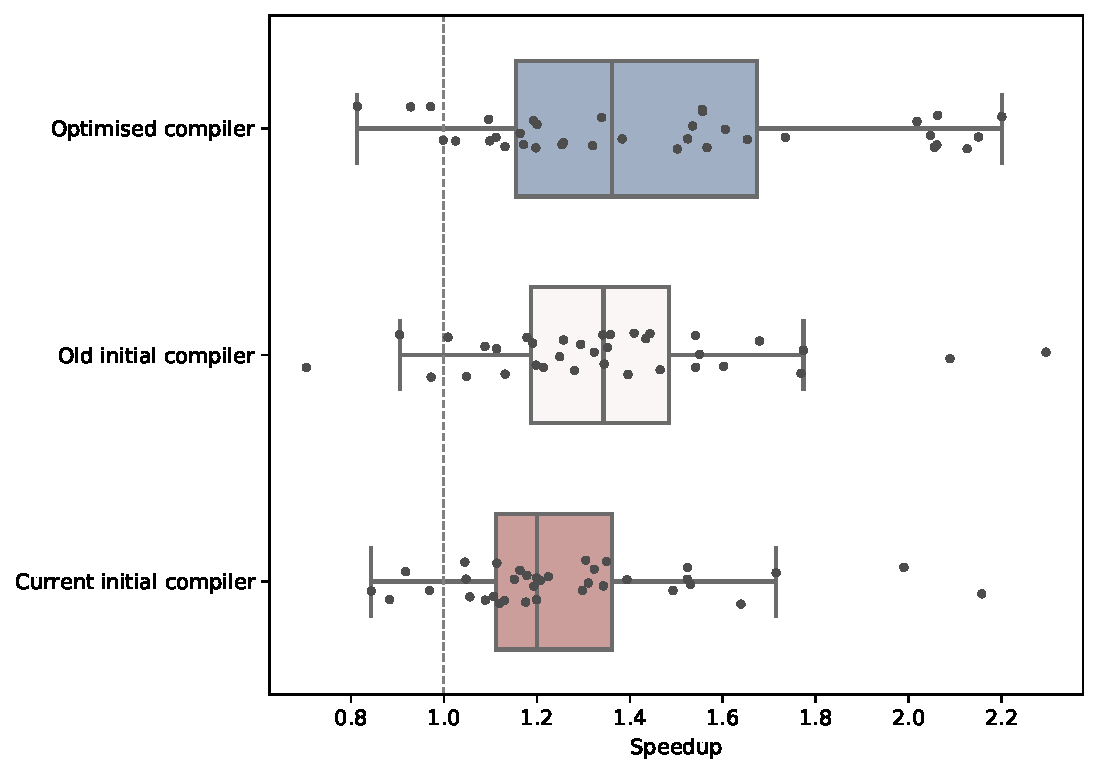
\includegraphics[width=\textwidth]{box}
    \caption{Distribution of speedup values for each version of the JIT}
    \label{fig:box}
\end{figure}

Figure \ref{fig:box} shows the high level summary of results on the execution speedup time. The
chart shows a standard box plot with points for each result overlayed. The points are vertically
offset randomly.

The general trend is of an increased execution time for most programs on all 3 compilers. The
initial compiler as it existed before the changes made in section \ref{dyn-recomp} was faster than
the current version. This is likely due to the the extra level of pointer indirection on function
calls to find the code pointer and overhead imposed by walking the stack on garbage collection.

The combination of the optimised compiler and current initial compiler version performed slightly
worse on programs in the lower half of the speed distribution  which can be seen by the decreased
lower quartile value.  However it had a slightly increased median and much better on the top half
of the distribution with a cluster of 8 programs managing to half the execution time relative to
the stock interpreter.

Although most programs tested benefited from the changes, about 5 programs did not and had
unchanged or decreased performance.

\subsection{Detailed results}

\begin{landscape}
    \begin{figure}[h]
        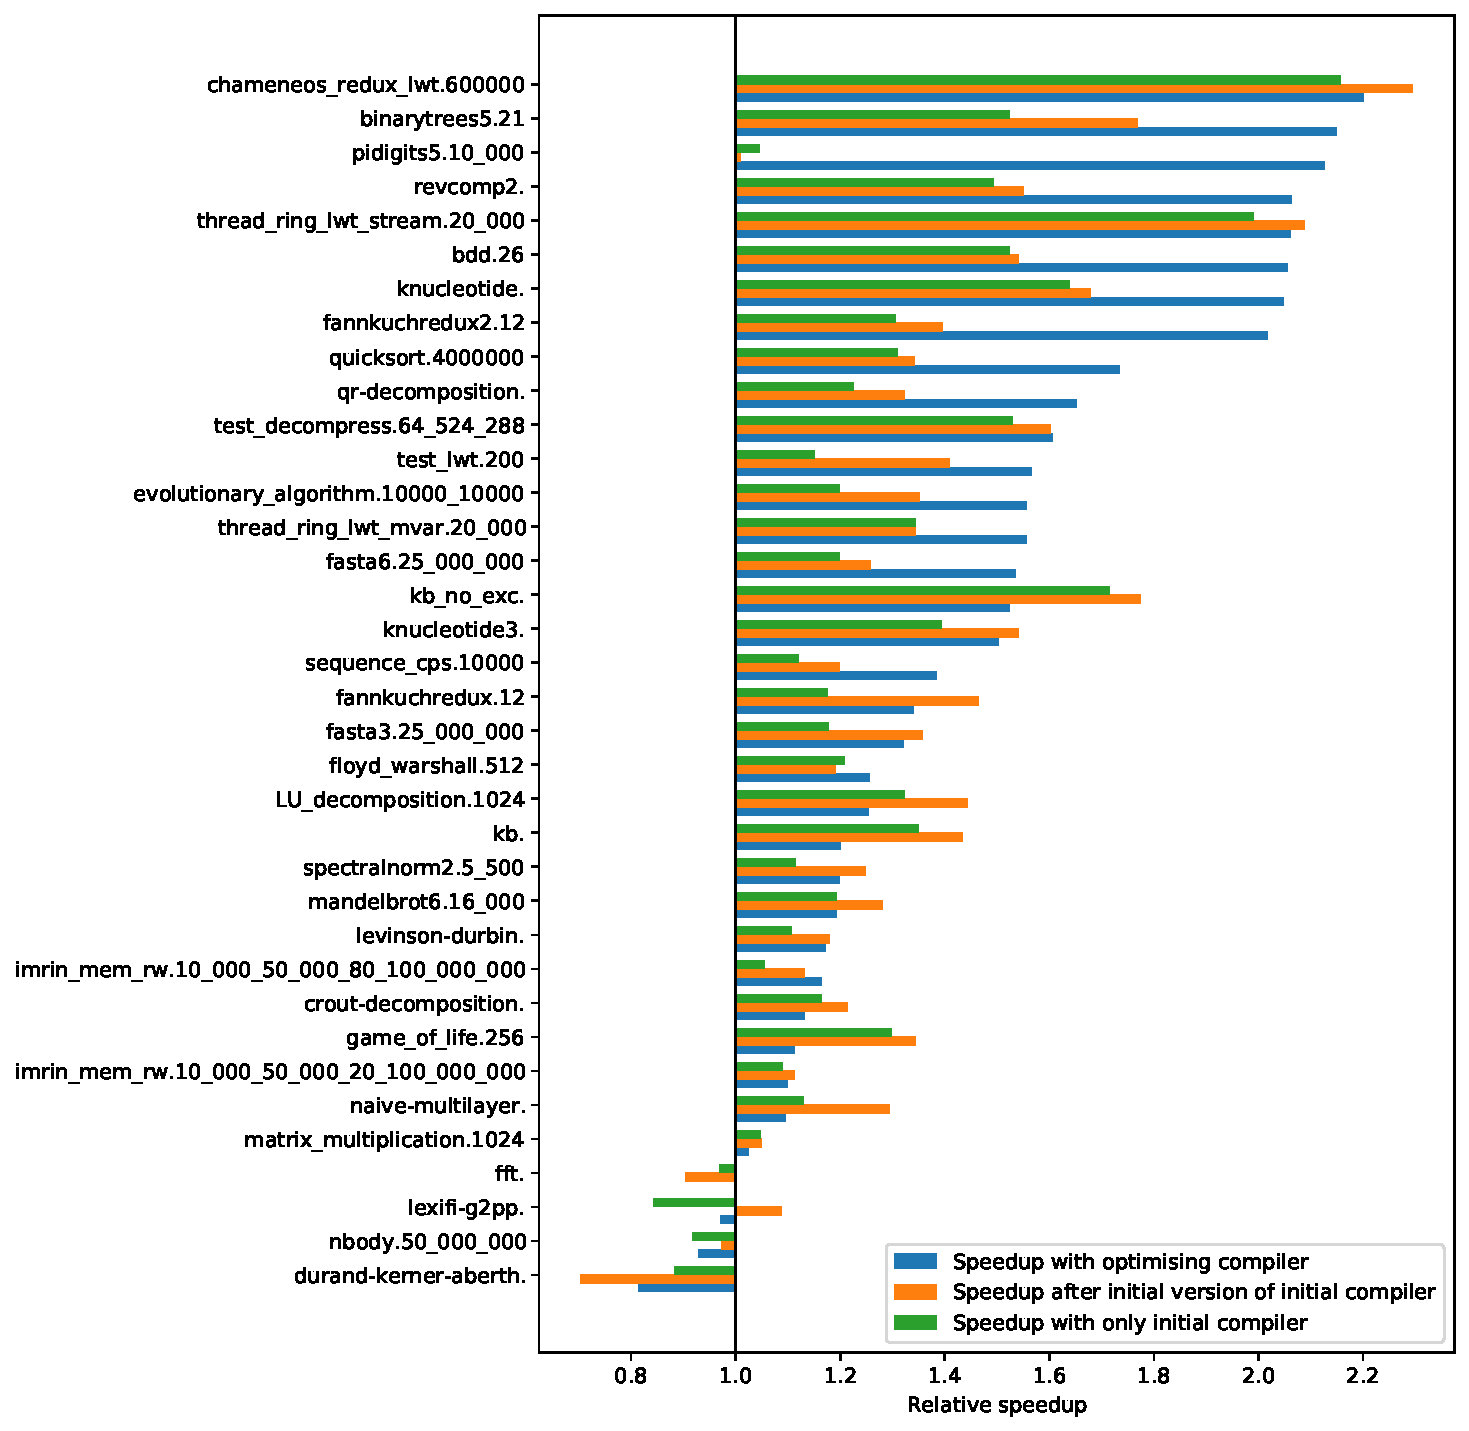
\includegraphics{perf}
        \caption{Speedup values for each benchmark}
        \label{fig:perf}
    \end{figure}
\end{landscape}

Show table of some results and graph of speedups. Mention distinction between tracing code + it
disabled.

\subsection{Overhead of supporting recompilation}

Show table/graph showing performance loss by extra indirection

\subsection{Optimised compiler}

Show table graph

\section{Evaluation of results and design trade-offs}

Write some stuff about when to use which compiler. Explain why certain ones were good/bad.

Quantify overhead for shorter running programs and explain it's likely to be slower. Use
self-hosting the compiler as a particularly bad case for the system.

Go into better cases for it and explain why it works. Possibly include code snippets.

\subsection{Bias}

The nature of the programs tested imposed some biases.

\subsubsection{Execution time}

Execution times ranged from \SI{1}{\second} to \SI{500}{\second}. Of the 36 benchmarks, 13 took
below \SI{10}{\second} and 7 took above \SI{50}{\second}.

In the context of these projects this means all programs classify as somewhat long-running and time
spent on compilation was a rather small goal.

\subsubsection{Work done}

Nearly all of the benchmarks included the same work being done many times in a hot loop. This is
the best
case for modern CPUs and dynamically optimising compilers.

Although the performance of programs is dominated by the hot path loops, larger programs tend to
also
have more cold code executed once or only a few times. The nature of the benchmarks means the
impact
of this is less well tested.

\section{Summary}

The initial compiler increased performance for most tested programs while retaining the semantics
and the
ability to run all OCaml bytecode programs.

Adding the optimised compiler led to significantly increased execution time on some tested programs
while decreasing the time for others.

The project met its success criteria early and was able to successfully implemented a significant
extension.